\documentclass[12pt]{article}
\usepackage{graphicx}
\usepackage{fullpage}
\usepackage{float}
\usepackage[symbol]{footmisc}
\graphicspath{{../images/}}
\usepackage{titlesec}% http://ctan.org/pkg/titlesec
\title{Radio Interferometry}
\author {
Kevin Yu
}

\begin{document}
\maketitle

\begin{abstract}
We use a radio interferometer to observe the Sun, the Moon, and 3C144 (the Crab Nebula). We fit an expression for the fringe amplitude to the data from our observation of 3C144. By using a brute force least-squares minimization algorithm, we measure the East-West baseline of our interferometer to be $10.06$ m. Using a similar procedure, we measure the declination of 3C144 to be $21^\circ 07' 26.8''$. Finally, we approximate the angular diameter of the Sun and the Moon by comparing the shape of the fringe's amplitude modulations to that of the theoretical Bessel function. We find the Sun's angular diameter to be $0.542^\circ$ and the Moon's angular diameter to be $0.548^\circ$. These values agree well with the known angular diameters of these bodies.
\end{abstract}

\section{Introduction}
Radio interferometry uses multiple radio receivers to construct a signal whose amplitude and frequency modulations give us information about a source. By correlating the signal received at the telescopes as the object moves across the sky, one observes a fringe pattern dependent on the angle between the interferometer baseline and the direction of the source. Fitting known functions describing this fringe to the data received allows us to make determinations of values such as the baseline of the interferometer and the declination of the source. In addition, for a circular source, amplitude modulations of the fringe reveal the angular diameter of the source.

In this report, we begin by discussing the basic concepts of interferometry and why we expect a interferometric fringe response when observing a source. Next, we discuss our method of observing objects, from locating them in the sky to tracking them using our equipment.

Using the data we collect for the 3C144, we perform least squares fitting to determine our baseline in the East-West direction and the declination of the 3C144.

Finally, we use the amplitude modulated fringe pattern of the Sun and the Moon in order to meausure their angular diameters. To do this, we compare the roots of the theoretical Bessel function describing the shape of the fringe envelope to the minima we observe in the envelope.

\section{The Interferometer}
The interferometer consists of two radio dishes separated along an approximately East-West baseline. Our baseline separation between the two dishes is approximately $B_y = 10$ m\footnote{We will measure this more precisely in Section 4}. We observe radiation at $10.67$ GHz, or $\lambda = 2.8$ cm wavelengths.

Interferometry depends on the time-delay between the detection of a plane wave at each receiver. This time-delay $\tau$ varies as the source moves across the sky and has two contributions: the geometrical difference in distance between the two detectors $\tau_g$ and the difference in cable length $\tau_c$.

Because we are on a E-W baseline, our geometrical time-delay is described by this expression:
\begin{equation}
\tau_g(h_a)= \frac{\mathbf{B} \cdot \mathbf{\hat{s}}}{c} = \left( \frac{B_y}{c} \right) \cos{\delta} \sin{h_a} \label{eq:geometric-delay}
\end{equation}
in which $\mathbf{B}$ is the baseline vector, $\mathbf{\hat{s}}$ is a unit vector in the direction of the source, $\delta$ is the declination of the object, and $h_a$ is the hour-angle of the object\footnote{This is a time-like coordinate, equal to the observer's local sidereal time minus the object's right ascension.}.
The output of the interferometer is the time average of the product of the signals received at each detector. When they are correlated and time averaged, the amplitude we observe due to the point source should be described by the following expression:
\begin{equation}
F(h_a) = \cos(2\pi \nu [\tau_g (h_a) + \tau_c]) \label{eq:fringe-output}
\end{equation}.
Because $\tau_g$ varies as the source goes through hour angles across the sky, this expression describes a sinusoidal \textit{fringe} pattern. Because $\tau_g$ is proportional to the sine of $h_a$, the rate that the $F(h_a)$ changes (the fringe frequency) depends on where it is in the sky; at the meridian the fringe frequency is greatest and at the horizon the fringe frequency will be the slowest. This can be seen a Taylor expansion of Eq. \ref{eq:geometric-delay}, which gives us the concept of a local fringe frequency---the fringe frequency seen when the source is at a particular hour angle:
\begin{equation}
f_f = \frac{B_y}{\lambda}	\cos{\delta} \cos{h_a} \label{eq:local-fringe-frequency}
\end{equation}

In Eq. \ref{eq:local-fringe-frequency}, $\lambda$ is the wavelength of our observed radiation. In order to make determinations of $B_y$, $\delta$, and $\tau_c$, we want to fit our observed fringes to Eq. \ref{eq:fringe-output}. Following the procedure of the lab manual, we can rewrite the fringe amplitude expression in this form:
The voltage we detect should be described by this expression:
\begin{equation}
F(h_a) = \cos{2\pi \nu \tau_c} \cos{\left( 2\pi \frac{B}{\lambda} 
\cos{\delta} \sin{h_a} \right)} - \sin{2\pi \nu \tau_c} \sin{\left( 2\pi \frac{B}{\lambda} 
\cos{\delta} \sin{h_a} \right)} \label{eq:fringe-amplitude}
\end{equation}
This equation is more suited than Eq. \ref{eq:fringe-output}  to the least squares fitting method that we will employ in Section 4, in which we will fit the constant coeffecients $ \cos{2\pi \nu \tau_c}$ and $ \sin{2\pi \nu \tau_c}$.

\section{Observing}
\subsection{Locating Objects}
The coordinates of celestial bodies are most often given in the equatorial coordinates of right ascension (RA) and declination (DEC). Right ascension is the object's angular distance eastward relative to the vernal equniox. Declination is the angle between the object and an axis parallel to the Earth's north pole. The coordinates are defined relative to the orientation of the Earth and do not change depending on one's location. However, they are not that useful to an observer who wants to track the object's motion as it travels across his or her sky.

To know where to point the telescope, we must translate our equatorial coordinates into altitude and azimuth, which represent a position on the sky relative to the observer. Altitude of $90^\circ$ is directly overhead, while altitude of $0^\circ$ is on the horizon. Azimuth represents what direction the source is relative to North, and is often represented in hours (0 hours is directly north, while 12 hours is directly south).

To get to altitude and azimuth, we first want to convert our right ascension into our local hour angle, HA. The hour angle is a time-like coordinate which is the difference between the observer's local sidereal time and the object's right ascension. The local sidereal time increases linearly and thus the hour angle is a time-like coordinate that describes the object's angular position relative to the observer rather than the vernal equniox.

From hour-angle and declination, we can apply rotation matricies based on the observer's latitude and longitude to rotate the coordinates to azimuth and altitude. Applying these transformations give us  coordinates which tell us how high an object is in the sky and what direction it is in, and we can point our telescopes toward it accordingly.

Another thing to note here is that because the Earth precesses slowly, the equatorial coordinates of RA and DEC will start to change over the years. Thus, right ascensions and declinations that we look up are recorded along with their \textit{epoch}, which provide a reference point as to what date those coordinates were valid. From that date, the coordinates can be adjusted to the current date.

In this lab, we will primarily use the Python module PyEphem, which handles the conversion to the current epoch as well as conversions from equatorial coordinate to (az, alt) with ease.

\subsection{Observation Targets}
We will observe 3C144 (the Crab Nebula), whose angular diameter is small enough that we can consider it a point source for our interferometer. We selected this source for the most part due to the fact that it is a relatively bright source at the wavelengths we are interested in.

Additionally, we observe the Sun and the Moon horizon-to-horizon, allowing us to see the fringe frequency and the fringe amplitude modulations over a span of hour angles. The phase of the Moon during the time of our observation was first quarter.

\subsection{Tracking Objects Using Interferometer}
In order to observe the changing fringe pattern across the sky, we intend to make observations of our radio sources as they cross the sky from horizon to horizon. In order to track them, we must repoint the telescopes regularly in order to keep the sources within our aperture, which has a width of about $1^\circ$.

Due to limitations of the telescopes, the two dishes cannot point to sources below $15^\circ$ or above $87^\circ$ in altitude. Thus, we can only make measurements while the target objects is within our telescope's range.

We originally took datasets while repointing our telescopes once every two minutes. However, these observations provided us with very poor results. The reason for this is likely the fact that the repointing frequency was too low; objects in the sky typically move about $1^\circ$ every four minutes. In two minutes time the target would have moved significantly to the edge of or even off of our aperture, and we lose the full signal until we repoint. 

We solved this by increasing the repointing frequency to once every thirty seconds. This allowed us to keep the target object within our aperture at all times and provided reasonable results. In addition to repointing the telescope, it is recommended that we home the telescope every hour or so due to rounding errors in each repointing. Moving to the \textit{home} position reduces pointing error, but also causes unusable sections of data which will be noticable in large spikes or changes in the signal.

\section{3C144}
Determinations of certain quantities can be determined by fitting Eq. \ref{eq:fringe-amplitude} to data from 3C144, which is a point source to our interferometer. This equation has three unknown quantities: the time delay due to differences in cable length, $\tau_c$, the baseline $B_y$, and the declination of the target, $\delta$. As we will see, if we assume our value of $\delta$ is accurate (as looked up in a catalog) we can use least squares fitting to determine our baseline $B_y$. Similarly, assuming a value for the baseline $B_y$, we can use a similar procedure to determine the actual declination of 3C144.

\subsection{Processing 3C144 Data}

\begin{figure}[H]
\center{
  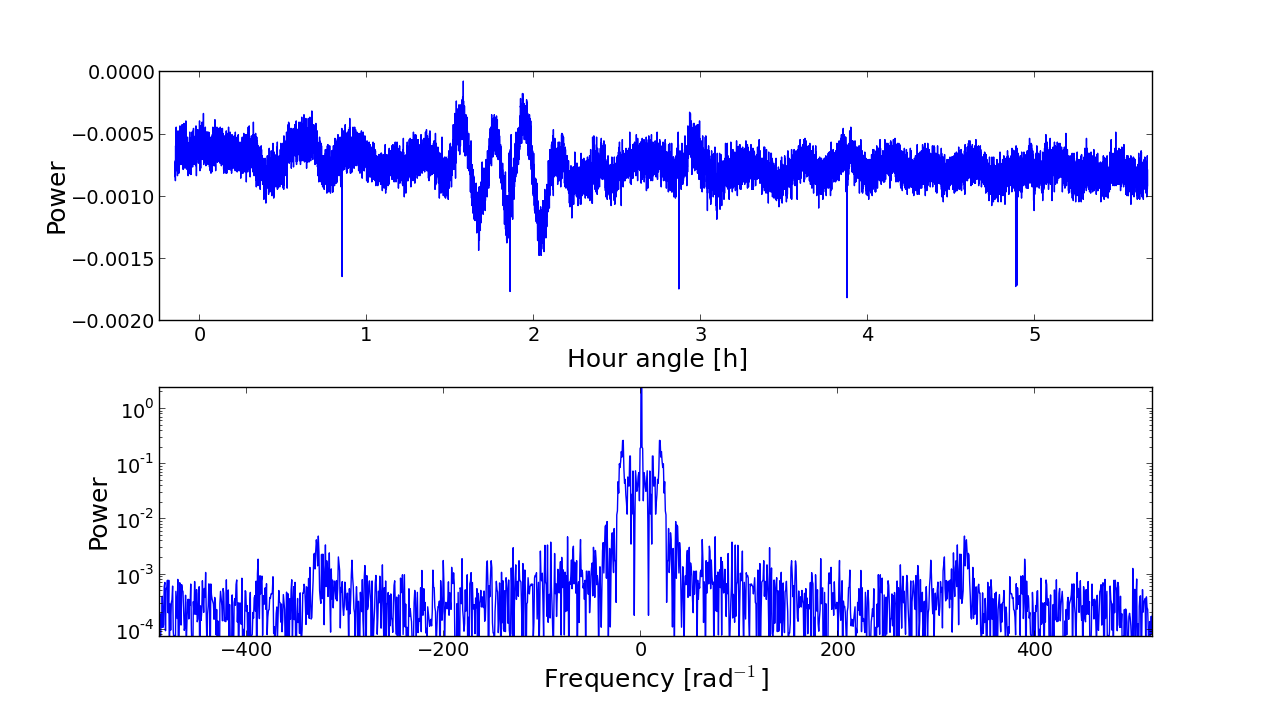
\includegraphics[width=440px]{original}
}
\caption[SODUMB]{Interferometric data taken for 3C144 on 4/3/2014. Data collection began just before 3C144 crossed the meridian.}
\label{fig:original}
\end{figure}

Figure \ref{fig:original} shows the signal collected for just about half of 3C144's transit across the sky. The data contains a lot of noise and has large, low frequency features that are inconsistent with the expected shape of the fringe; from Eq. \ref{eq:fringe-output}, the signal of our source should simply be a sinusoidal wave of about constant amplitude and varying frequency. Additionally, there is a clear DC component to the signal. These components of our signal must be removed before fitting can be done.

To extract the signal we are interested in, we first will use the technique of Fourier Filtering to eliminate frequencies which we know should not be seen in the 3C144 signal. We can remove frequency components by transforming to the frequency domain, eliminating unwanted frequencies, and then applying an inverse fourier transform back into the time domain.

The frequency range which we will attempt to extract will be determined by the range of fringe frequencies we expect by Eq. \ref{eq:local-fringe-frequency}. The fringe frequency reaches a maximum value where $|\cos{\delta} \cos{h_a}|$ is a maximum. The same reasoning applies to the minimum fringe frequency. For our observation of 3C144, these extrema occur at the following fringe frequencies:
\begin{eqnarray}
f_{f, max} = 371\ rad^{-1}\\
f_{f, min} = 32\ rad^{-1}
\end{eqnarray}
We apply a bandpass Fourier filter to our data that removes frequency components less than $f_{f, min}$ and greater than $f_{f, max}$.

Because the function that we will be fitting to can be written as Eq. \ref{eq:fringe-output}, the main goal of fitting here is to fit $\delta$ or $B_y$ such that the fringe frequency matches the data. However, it is clear from Figure \ref{fig:filtered} that our fringe contains modulations in amplitude. This causes a problem in least-squares fitting as the amplitude modulations will affect the fit when in fact the most important aspect we would like to fit is the frequency.

We solve this issue by normalizing the data in bins of 200 data points to the maximum value in each bin. For most of the dataset, this brought the data to approximatly the same amplitude which allowed us to fit the fringe. However, as you can see from the time domain signal, this method of normalizing is susceptible to amplifying noise more in some sections of the data when there are outliers and in particular this occurs every hour where we homed the telescope. However, because the telescope homing is not a huge part of the dataset, it should not affect our fit too badly.

Using this technique of normalizing to the amplitude of nearby points turns out to be extremely important in successfully fitting a the fringe amplitude to the data, and allows us to make good meaurements of both our interferometer's baseline and the declination of 3C144. The resulting signal and its power spectrum are shown in Figure \ref{fig:filtered}.

\begin{figure}[H]
\center{
  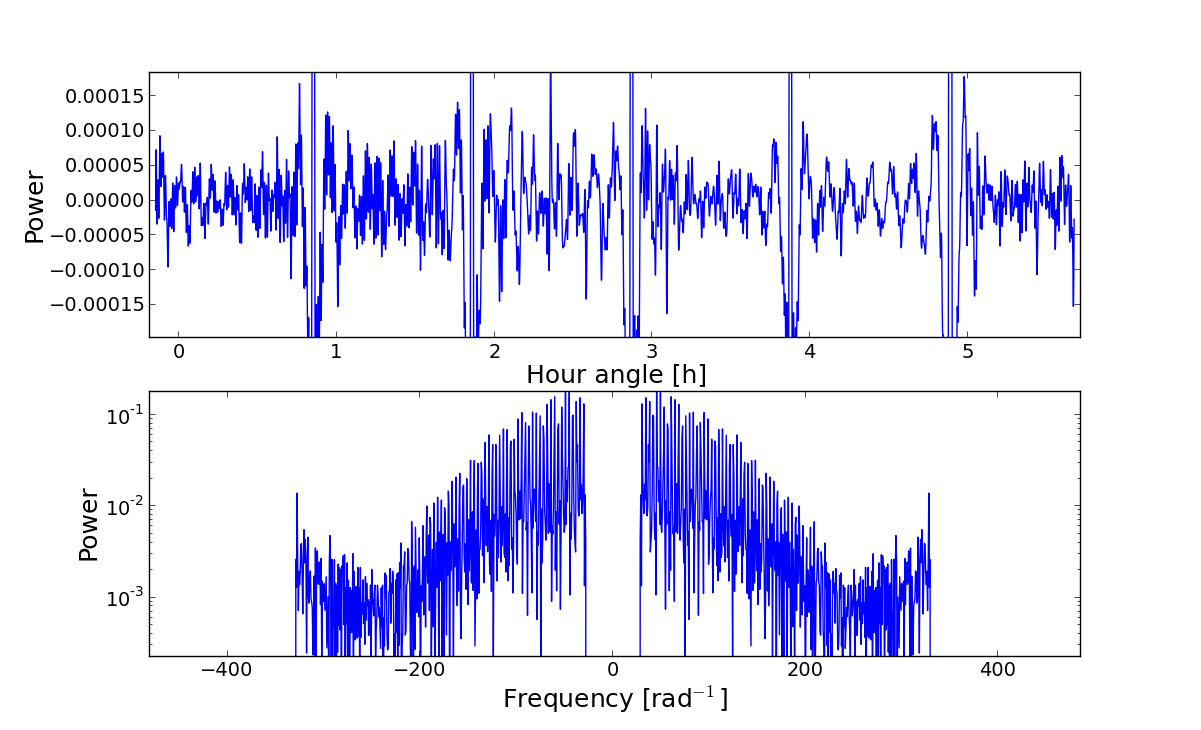
\includegraphics[width=440px]{filtered}
}
\caption[SODUMB]{Data for 3C144 after filtering out frequencies greater than the maximum fringe frequency and slower than the minimum fringe frequency. The DC offset is removed. Spikes at each hour occur due to homing of the telescope and may have been exaggerated by the normalization methods used.}
\label{fig:filtered}
\end{figure}

\subsection{Fitting the Baseline}
For purposes of determining the baseline using 3C144, we use the documented declination of $\delta_{J2000} = 22^\circ 00'52.1'' = 0.3842$ rad. The precessed value of this declination in the current epoch is $\delta_{today} = 22^\circ 04'14'' = 0.3852$ rad.

A least squares method can be used on the filtered and normalized data of Figure \ref{fig:filtered}. The method we use to fit the baseline is as follows:

\begin{enumerate}
  \item We rewrite Eq. \ref{eq:fringe-amplitude} with constant coefficients filled in for the $\tau_c$ dependent factors. 
  \begin{equation}
F(h_a) = C_1 \cos{\left( 2\pi \frac{B_y}{\lambda} 
\cos{\delta} \sin{h_a} \right)} - C_2 \sin{\left( 2\pi \frac{B_y}{\lambda} 
\cos{\delta} \sin{h_a} \right)} \label{eq:fringe-amplitude}
\end{equation}

  \item To fit $B_y$, we iterate over a range of possible baseline values and apply a linear least-squares fit using each one. From the lab manual, we know that the baseline is near $10$ m; however, we probe values of $B_y$ ranging from $5.00$ m to $15.00$ m in order to demonstrate the efficacy of this method. We try values of $B_y$ in steps of $0.01$ m; this step size limit sthe resolution at which we can determine the baseline.
   \item We look at the $\chi^2$ values for each of the linear fits performed in the last step. The baseline value corresponding to the smallest value of $\chi^2$ is our best fit baseline.
\end{enumerate}

\begin{figure}[H]
\center{
  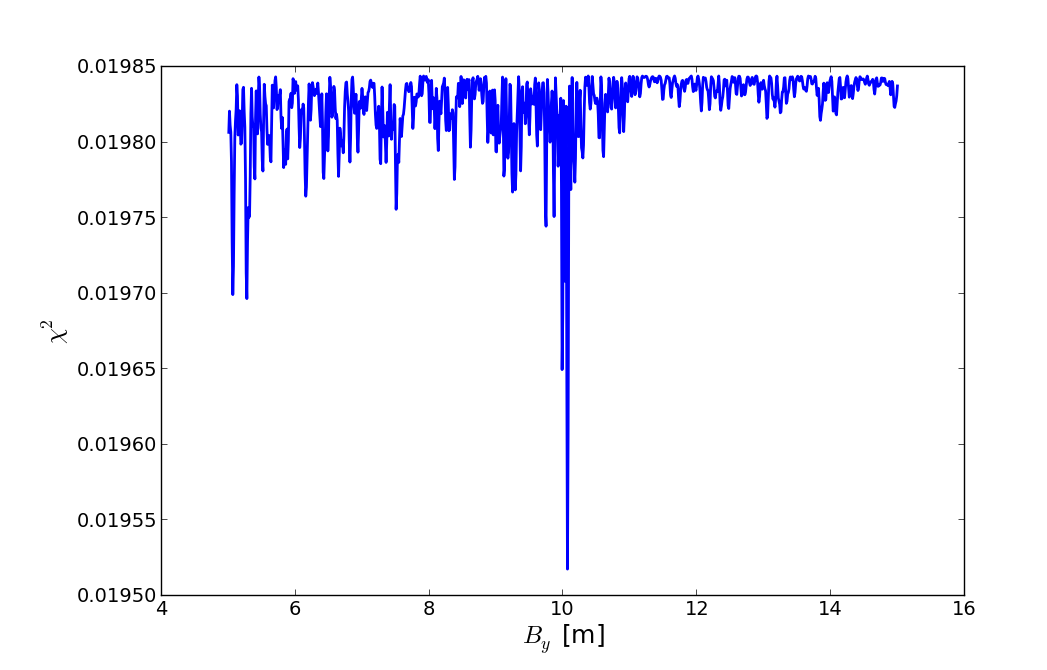
\includegraphics[width=380px]{baseline_chi2}
}
\caption[SODUMB]{The $\chi^2$ values of linear fits for various values of $B_y$. The $\chi^2$ value, which is defined as the sum of the squared residuals between the fit and the observations, divided by the degrees of freedom in each fit. It is minimized at $B_y=10.06$ m.}
\label{fig:baseline-chi2}
\end{figure}

By applying the above procedure, we find a range of $\chi^2$ plotted in Figure \ref{fig:baseline-chi2}. There is a single point that clearly minimizes the $\chi^2$ of the fit; this is our measurement of the baseline:
\begin{equation}
B_y = 10.06\ m 
\end{equation}
Before moving on, allow me to point out the importance of normalizing the data. Without normalizing the data and leaving the amplitude fluctuations, the array of $\chi^2$ for the very same baseline values appears as in Figure. \ref{fig:bad-chi2}. Not only is the measurement of $B_y$ significantly off, there are also many comparable local minima which leaves a lot of uncertainty as to the true value of $B_y$.

\begin{figure}[H]
\center{
  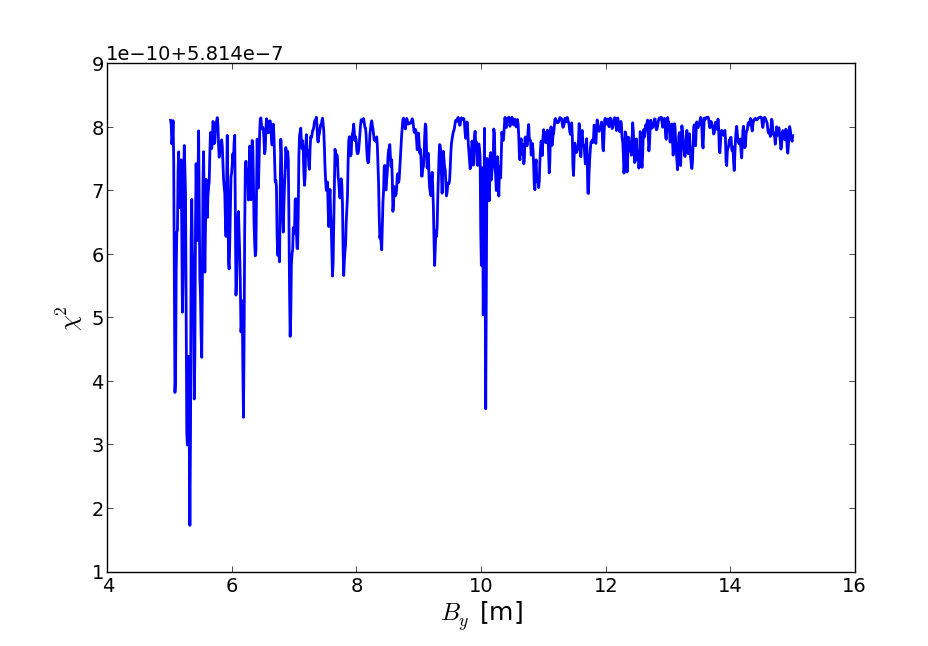
\includegraphics[width=350px]{bad_chi2}
}
\caption[SODUMB]{The $\chi^2$ values of linear fits for various values of $B_y$, using \textit{unfiltered and unnormalized data}. There is a local minima at $B_y=10.06$ m, but due to noise and other contributions, there are many comparable spikes in $\chi^2$ and in fact is minimzed in this range by $B_y \approx 5.3$ m. It is clear that filtering and normalization was necessary to properly fit the data.}
\label{fig:bad-chi2}
\end{figure}

\subsection{Declination of 3C144}
We now take the baseline length of $B_y = 10.06$ m as a truth of reality and will fit the declination using the same method as above. Instead of probing different baseline values, we probe different values of the declination to minimize the square residuals.

Knowing that the declination should be around $22^\circ$, we will try values of $\delta$ from $12.00^\circ$ to $32.00^\circ$ in steps of $0.01^\circ$. The $\chi^2$ values for these declinations are shown in Figure \ref{fig:dec-chi2} and the best fit value for the declination is:
\begin{equation}
\delta_{3C144} = 21^\circ 07'26.8''
\end{equation}
This measurement is reasonably close to the PyEphem calculated value of $\delta_{J2000} = 22^\circ 04'14'' $. 

\begin{figure}[H]
\center{
  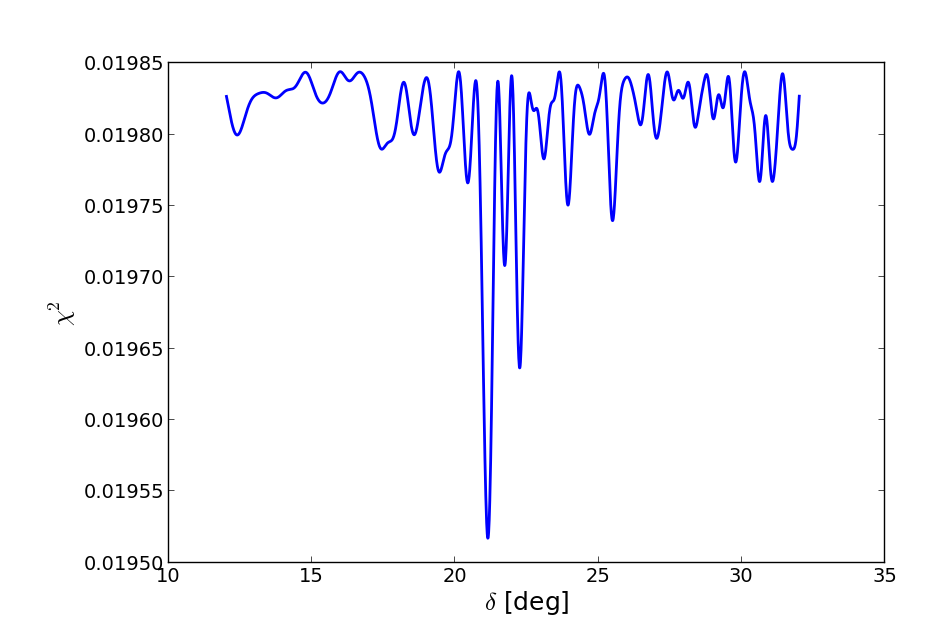
\includegraphics[width=380px]{dec_chi2}
}
\caption[SODUMB]{The $\chi^2$ values of linear fits for various values of $\delta$, using the same method as for the baseline. The $\chi^2$ value is minimized for $\delta = 21.12^\circ$. There is a bit of uncertainty here due to the fact that another value of $\delta$ near $23^\circ$ has a comparable local minima in $\chi^2$.}
\label{fig:dec-chi2}
\end{figure}

\section{The Sun}
Sources whose brightness span an angle in the sky (i.e. not point sources) contain additional information in the fringe amplitude. The data collected is the integral of the entire object multipled by the fringe amplitude.

The Sun's intensity as a function of angular separation from its center can be described by the following equation:
\begin{equation}
I(\delta h ) = \frac{(R^2 - \Delta{h}^2)^{1/2}}{R} \label{eq:sun-intensity}
\end{equation}
Here, R is the angular radius of the source. The data that we observe of the Sun is essentailly integrating the product of this intensity and the fringe, over the hour angles the Sun spans. By simplifying the integral, the interferometer response can be described as the product of the local fringe at the position of the sun modulating an envelope function $MF$. Generally, $MF$ is the fourier transform of the brightness distribution of the source on the sky.

Using Eq. \ref{eq:sun-intensity} in $MF$, which applies to a uniform and spherical source, we find that $MF$ is expected to be described by:
\begin{equation}
MF_{theory} = \frac{1}{R} \int_{-R}^{R} (R^2 - \Delta{h}^2)^{1/2} \cos{(2\pi f_f \Delta{h})} d\Delta{h}
\end{equation}
In order to evaluate the integral numerically, we rewrite this as a summation:
\begin{equation}
MF_{theory} \approx \sum_{n=-N}^{n=+N} \left[ 1- \left( \frac{n}{N} \right) ^2 \right]^{1/2} \cos{\frac{2\pi f_f R n}{N}}
\end{equation}

By comparing the theoretical $MF$ to our observations of the modulations in amplitude, we can make a determination of the angular radius of the Sun.

\begin{figure}[H]
\center{
  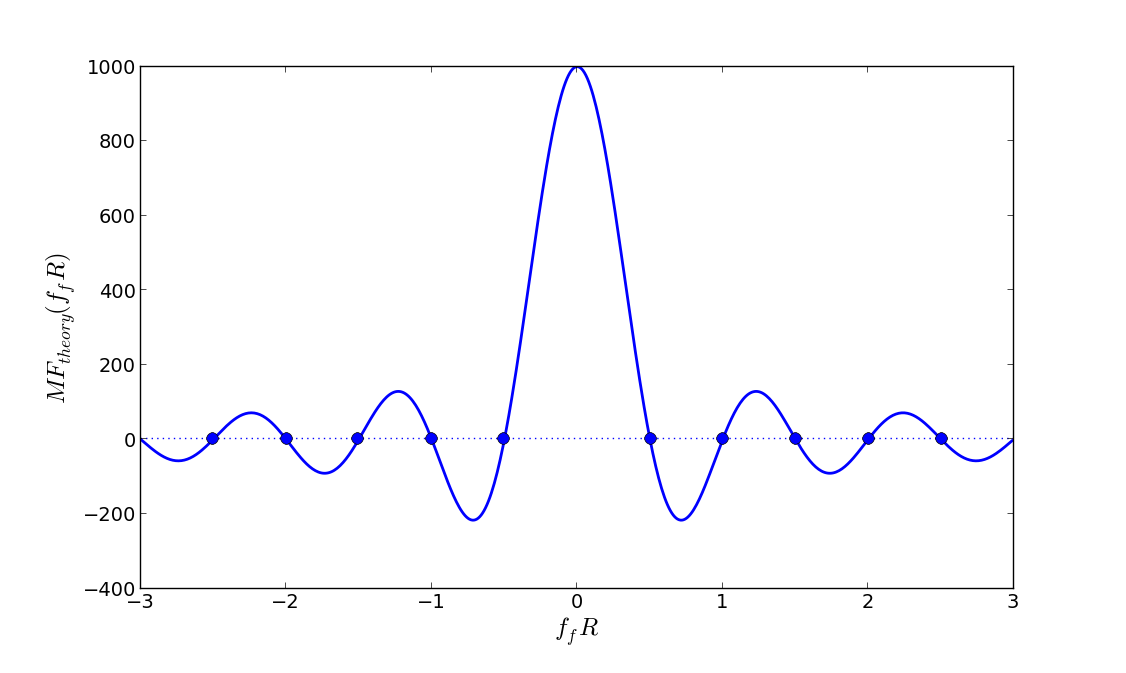
\includegraphics[width=440px]{MF}
}
\caption[SODUMB]{Theoretical $MF$ as a function of the quantity $f_f R$. It is a Bessel function whose zeros occur at known values of $f_f R: [ \ 0.60975\  1.11675\  1.61925 \ 2.12075\  2.62125\ \ldots\ ] $. By observing the fringe frequency at which the modulated envelope is minimized, we can determine the corresponding values of $R$.}
\label{fig:MF}
\end{figure}

\subsection{Measuring Solar Diameter}
The Sun's intensity allows our signal to generally overwhelm the noise of the system. The shape of the bessel-function envelope can already be seen even in the unreduced dataset (Figure \ref{fig:sunoriginal}).

\begin{figure}[H]
\center{
  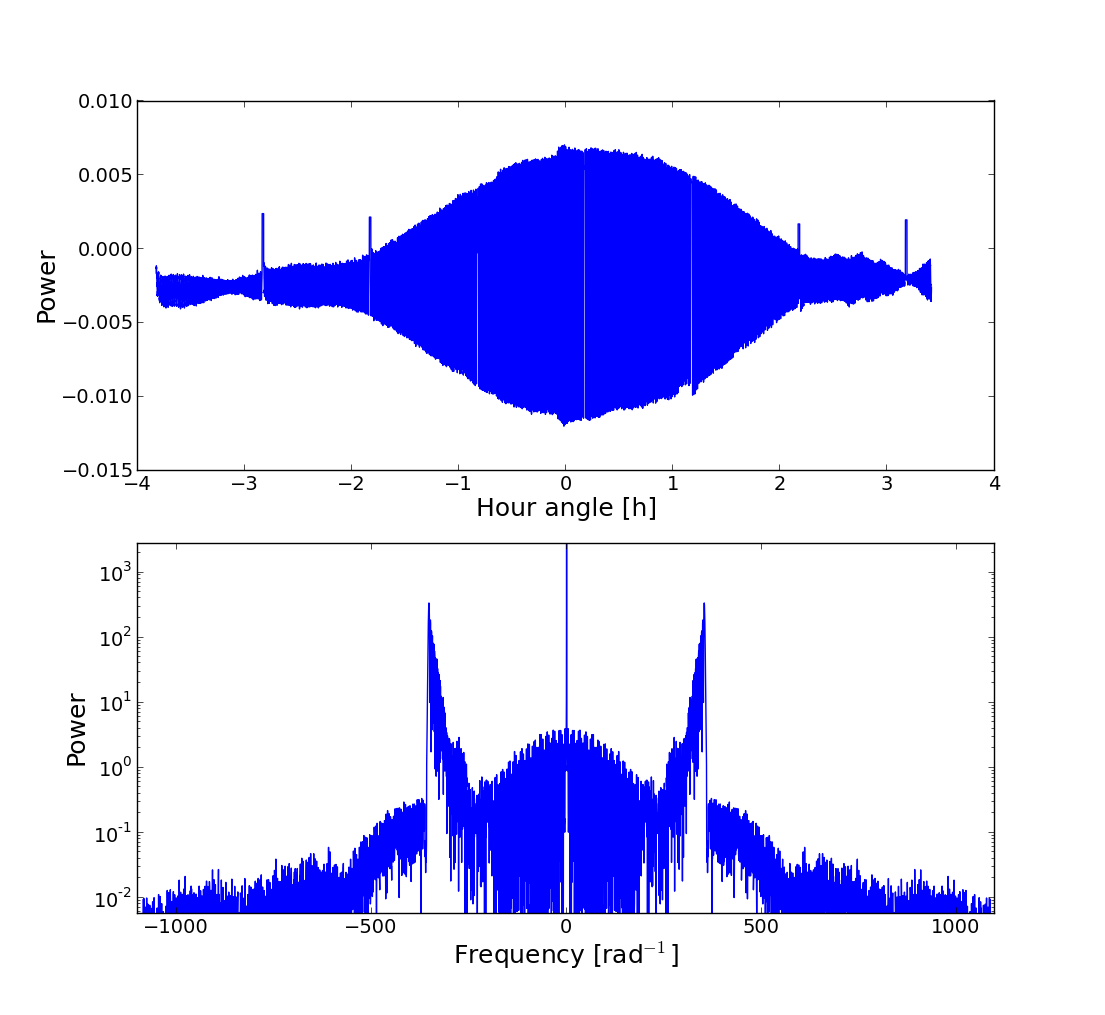
\includegraphics[width=440px]{sunoriginal}
}
\caption[SODUMB]{Raw data for the Sun taken on 4/3/2014, horizon to horizon. The sun's fringe frequencies can be seen in the spikes on either side of 0 rad$^{-1}$ in the power spectrum.}
\label{fig:sunoriginal}
\end{figure}

Similar, to the data for 3C144, we can determine the highest fringe frequency we expect and filter out noise higher than that frequency. Additonally, we even out the fluctuations by applying a filter in which we subtract from each point by the median of the surrounding 200 points. This will help center some sections of the data on zero without damaging the overall shape of the envelope, which is important in determining the angular radius of the Sun. The result of this filter is seen in Figure \ref{fig:envelope}.

To determine the angular diameter of the Sun, we note that the theoretical $MF$ is a function of the quantity $f_f R$, and has zero crossings at certain values as shown in Figure \ref{fig:MF}. These roots of this function are as follows:
\begin{equation}
f_f R = [ \ 0.60975\  1.11675\  1.61925 \ 2.12075\  2.62125\ \ldots\ ] \label{eq:fRs}
\end{equation}
We next determine the hour angles $h_a$ at which the envelope reaches a minimum---this corresponds to one of the zeroes of the Bessel function. At this values of $h_a$, we can compute the corresponding local fringe frequency using Eq. \ref{eq:local-fringe-frequency}. With this fringe frequency, we can divide the values in Eq. \ref{eq:fRs} by that fringe frequency to get the possible values of $R$ suggested by the data.

To determine the aforementioned values of $h_a$, we begin by extacting the envelope. To do this, we divide the dataset into bins of 50 data points each replace each bin with a point equal to the maximum of the absolute value of points in the bin. As long as the size of the bins is small enough to preserve the overall shape and features of the envelope, but large enough to span at least one period of the fringe, the resulting data points will represent the envelope with the proper magnitude. The result of this envelope detection method is shown in Figure \ref{fig:envelope}.

\begin{figure}[H]
\center{
  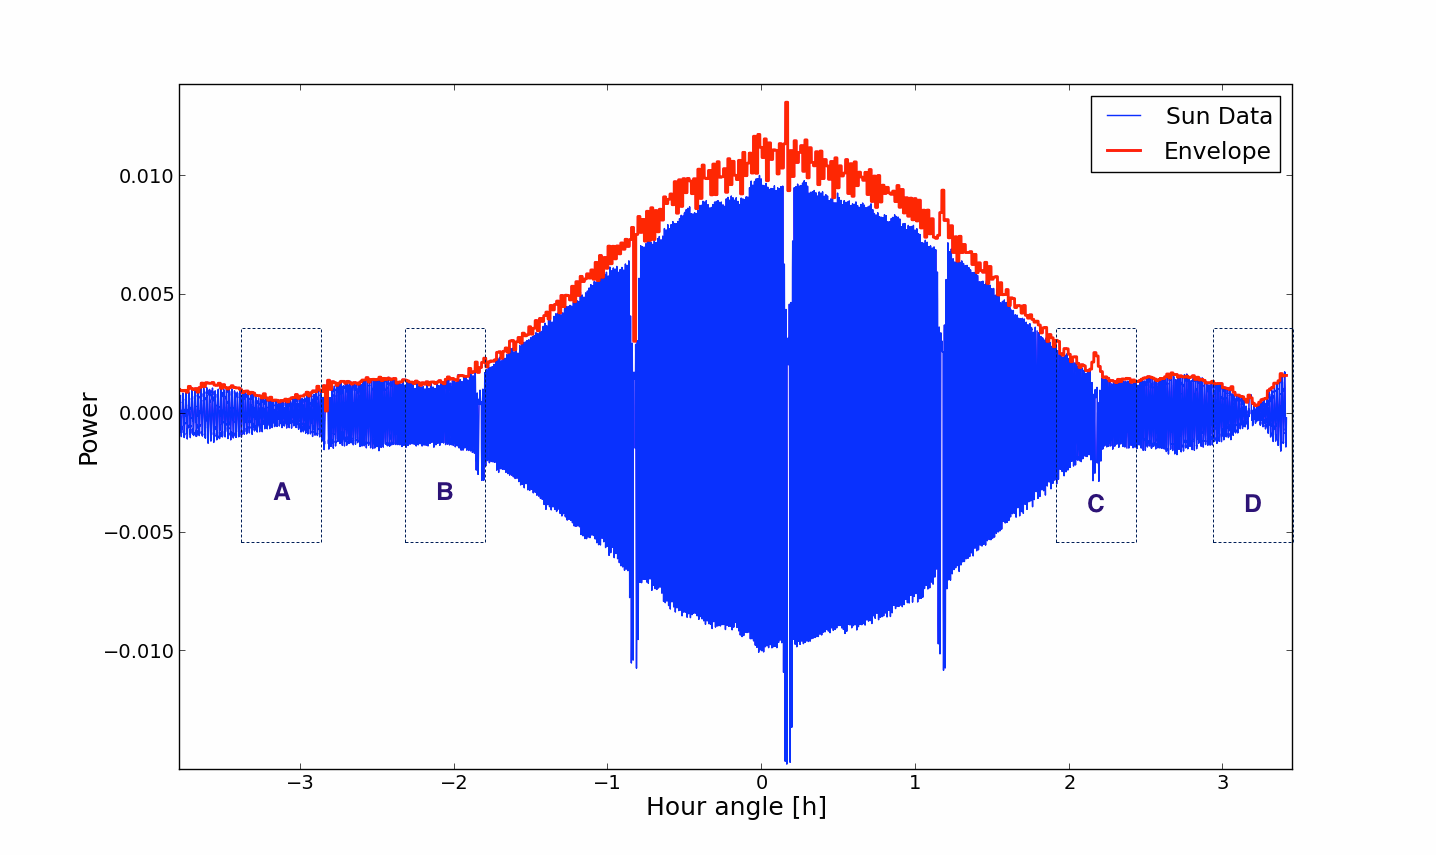
\includegraphics[width=440px]{envelope}
}
\caption[SODUMB]{Filtered data for the sun after removing the DC component of the signal and subtracting from each point the median of the 200 surrounding points. The envelope as extracted using the described method is shown in red slightly above the signal. Small spikes due to data taken while homing the telescope should be ignored and will not impact the fits very much. Minima in the envelope can be seen at points labeled by A, B, C, and D.}
\label{fig:envelope}
\end{figure}

By inspecting the shape of the envelope, we see minima marked by the circles in the plot. At each one, we can take a small slice of the envelope and fit a second order polynomial to the region. The minimal value of this fitted polynomial is is the hour angle of the zero crossing. A more robust method of fitting to the envelope would be to fit the fringe amplitude modulated by a high order polynomial to find the local minima. However, because of time constraints and the fact that there are only a few minima, this method of fitting second order polynomials to the envelope at locations of interest should suffice.

As can be seen in Figure \ref{fig:envelope}, the two minima labelled B and C are not well defined and are very shallow. In contrast, the crossings further out labelled A and D (at about $\pm3$ h) are more clearly defined, so I choose those for analysis\footnote{I will go back to the first crossing later and we find that it raises some questions.}. Fitting a second order polynomial to the two regions show that minima occur at $-3.214$ h and at $3.238$ h; reassuringly symmetric about the meridian. The corresponding fringe frequencies determined using Eq. \ref{eq:local-fringe-frequency} are listed in the following table, as well as the values of $R$ that allow that zero crossing by diving $f_f$ by the values in Eq. \ref{eq:fRs}:
\begin{table}[H]
\begin{center}
  \begin{tabular}{c | c | c }
    $h_a$ [h] & $f_f$ [rad$^{-1}$] & Possible $R$ [deg]\\ \hline
    -3.214 & 237.345 & [ 0.147  0.270  0.391  0.512  ... ] \\
    3.238 & 235.643 &  [ 0.148  0.272  0.394  0.515  ... ] \\
    \end{tabular}
\end{center}
\caption{Values of R that give an angular diameter of greater than $1^\circ$ can be ignored because that is approximately the limit of our telescope's aperture.}
\label{tbl:firfrequencies}
\end{table}

If we assume that these represent the second minima out from $h_a=0$ (and admittedly being reinforced by our prior knowledge of the angular size of the Sun) then our result for the angular diameter of the Sun is
\begin{equation}
D = 2R = 0.542^\circ \nonumber \label{eq:size-of-sun}
\end{equation}

However, assuming this is the second zero crossing is a bit problematic because it requires two more zero crossings (one positive, one negative) closer to zero. As we saw in Figure \ref{fig:envelope}, these local minima in the envelope are not as well defined and it is harder to determine at what hour angle they occur at. However, by fitting a second order polynomial to these regions, we find that minima occur at roughly $-2.312$ h and $2.476$ h. Assuming these correspond to the smallest roots of $MF$, the corresponding diameter measurements are $D = 0.239^\circ$ and $D = 0.246^\circ$, which are a factor of two off of the actual value.

Thus it is hard to confidently say that the measurement of $D = 0.542^\circ$ is totally valid, due to the missing node predicted $MF_{theory}$. However, it is clear that the shallower minima are largely affected by noise and possibly other non-uniform contributions to the Sun's brightness distribution, and the only zero-crossings that are trustworthy are the two that give us the result in Eq. \ref{eq:size-of-sun}.

\section{The Moon}
Reduction of data for the Moon follows closely that of the Sun. The mathematical basis behind determining the angular diameter of the Moon is identical to the analysis done in the previous section on the Sun if we assume the Moon is a uniform circular source.

However, power receieved from the Moon is much lower and thus the dataset will contain more noise. While the Sun's Bessel-like envelope in Figure \ref{fig:sunoriginal} was apparent without any reduction, the Moon's envelope is not very clear in Figure \ref{fig:moonoriginal}.

The procedure in reducing the Lunar data is identical, however. We first filter out unwanted frequencies greater than the range of fringe frequencies we expect, and then apply a filter which subtracts from each point the median of its surrounding 200 points. The result, and the extracted envelope can be seen in Fig. \ref{fig:moonenvelope}. Though it is harder to locate minima, there appears to be one at the location labelled by A where the envelope nears zero. Our confidence that this is actually a minima of the envelope rather than noise is bolstered by the fact that there appears to be a minima on the opposite size of the meridian at $h_a\approx 3$, consistent with a symmetric envelope.

\begin{figure}[H]
\center{
  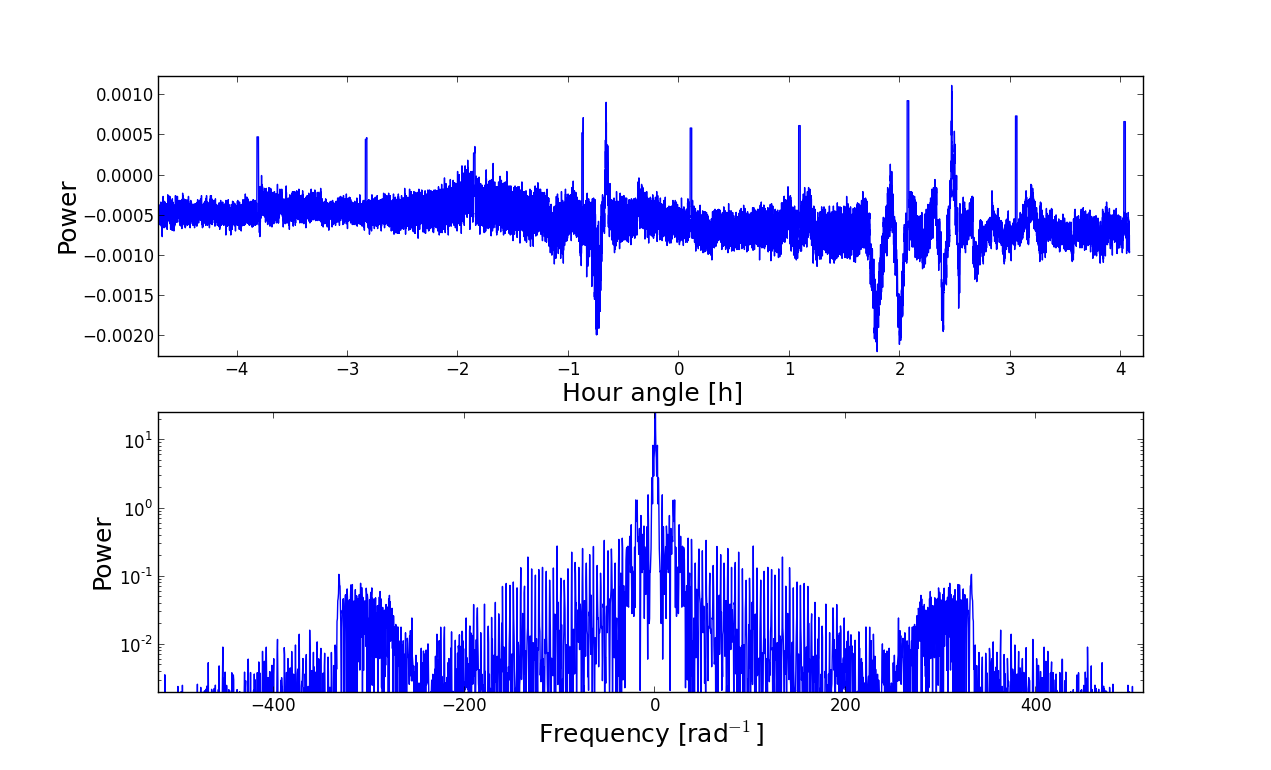
\includegraphics[width=440px]{moonoriginal}
}
\caption[SODUMB]{Raw data and spectrum for the Moon taken on 4/6/2014, horizon to horizon. The fringe frequencies can be seen in the spectra on either size of 0 rad$^{-1}$ but are not as strong as in the Sun data.}
\label{fig:moonoriginal}
\end{figure}

\begin{figure}[H]
\center{
  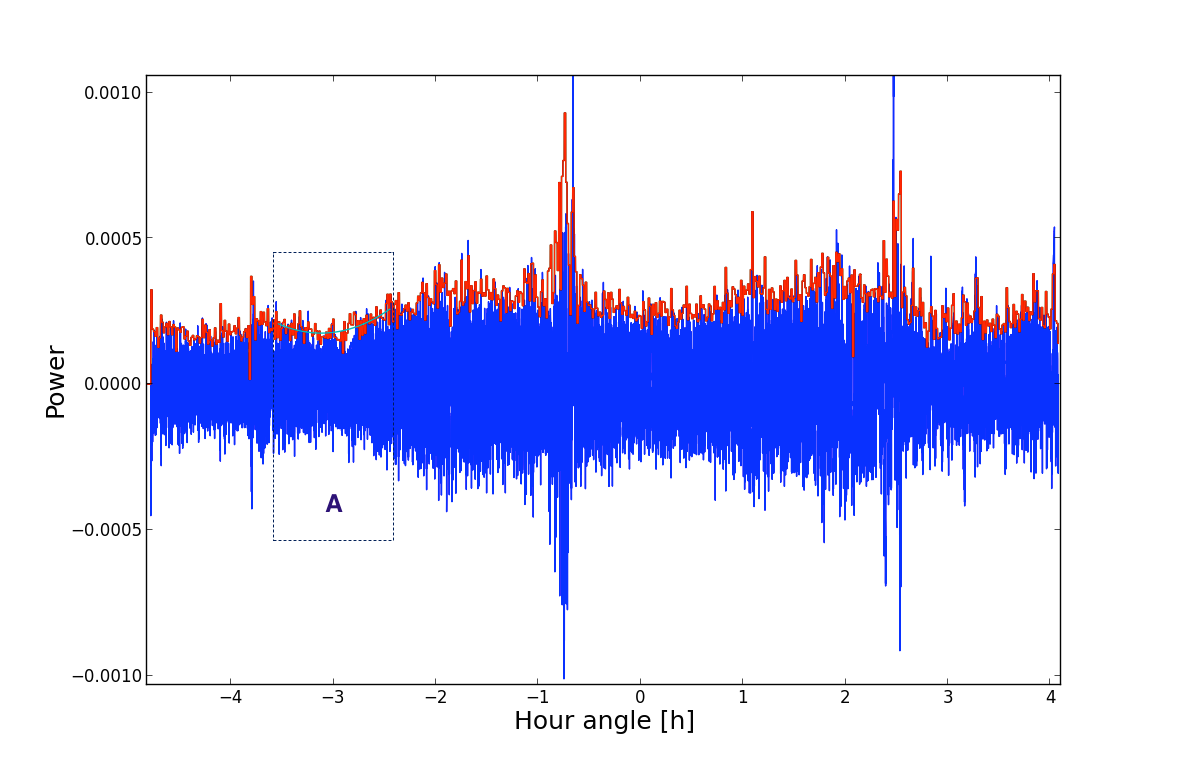
\includegraphics[width=440px]{moonenvelope}
}
\caption[SODUMB]{Filtered data for the moon after removing the DC component of the signal and subtracting from each point the median of the 200 surrounding points. The envelope as extracted using the described method is shown in red slightly above the signal. Although it is not as prominent as in the Sun data, there can be seen a minima where the envelope nears zero in the region labeled by A.}
\label{fig:moonenvelope}
\end{figure}

Using that datapoint, the possible values of R this describes are as follows
\begin{table}[H]
\begin{center}
  \begin{tabular}{c | c | c }
    $h_a$ [h] & $f_f$ [rad$^{-1}$] & Possible $R$ [deg]\\ \hline
    -3.122 & 233.56 &  [ 0.150  0.274 0.397 ...] \\
    \end{tabular}
\end{center}
\end{table}
Unlike for the Sun, in Figure \ref{fig:moonenvelope} it hard to tell whether our zero-crossing is the first, second, or third minima of the envelope. The most we can conclude from this is that the angular radius approximately among the possible values listed in the Table above. However, knowing that the moon's angular size is approximately the same as the Sun's, we can guess that the correct measurement here is $R_{moon}\approx 0.274^\circ$. The possible values of the Moon's angular diameter are\footnote{Excluding diameters greater than $1^\circ$, the aperture of the telescope.}:
\begin{equation}
D_{moon} = 2 R_{moon} = 0.300^\circ,\ \mathbf{0.548^\circ},\ 0.794^\circ
\end{equation}

\section{Conclusion}
In reducing inteferometric data, we find that subtracting a boxcar filtered signal from the original signal is extremely helpful in extracting the underlying signal. This can be done by subtracting from every datapoint the median of the surrounding points, which ``flattens" the signal and makes the amplitude of the signal clear.

We find that analysis of the point source 3C144 is greatly benefitted by the methods of filtering, which allows us to make measurements of the baseline of our interferometer as well as the declination of 3C144. Although the large amount of noise in the signal makes it impossible to make a very good fit, certain values for the baseline and declination can give a \textit{relatively} good fit compared to other values. This allows us to make measurements of our baseline ($B_y = 10.06$ m) and the declination of 3C144 ($\delta_{3C144} = 21^\circ 07'26.8''$). It is possible that our fits could be further improved by filtering in a way that does not cause the spikes due to telescope homing to become exaggerated.

In analyzing the data for the Sun and the Moon, we find that similar methods of data reduction allow us to see the shape of the envelope which should be described by a Bessel function. Because the Sun is so bright, its signal overwhelemed the noise and one of the zero crossings was very obvious, giving us an acceptable value of the Sun's diameter of $0.542^\circ$. Using the same methods for the Moon was more difficult to the smaller signal to noise ratio; however, by using one of the more prominent minima in the envelope, we find that the Moon's angular diamater is about $0.548^\circ$.

Sources of error are backgroud noise as well as inaccuracy in pointing the telescope. We find that it is necessary to repoint the telescope in a time much lower than it takes for the object to move across the aperture of the telescope; otherwise we may see amplitude modulations and distortions in the expected envelope for circular sources.

\section{Acknowledgement}
I would like to thank the lab instructors Aaron Parsons, Karto Keating, and Baylee Bordwell assisting us with analysis code and debugging observations, as well as my classmates for providing helpful discussion in figuring out the data analysis sections of the lab. 
All figures in this paper were done in Python using the Numpy and Matplotlib libraries. Location of targets were calculated using PyEphem module.

\end{document}